\documentclass{article}

\usepackage{fullpage}
\usepackage[round]{natbib}
\usepackage{multirow}
\usepackage{booktabs}
\usepackage{tabularx}
\usepackage{graphicx}
\usepackage{float}
\usepackage{xr}
\usepackage{xr-hyper}
\usepackage{hyperref}
\hypersetup{
    colorlinks,
    citecolor=blue,
    filecolor=black,
    linkcolor=red,
    urlcolor=blue
}

\usepackage[round]{natbib}
\usepackage{longtable}
\usepackage[utf8]{inputenc}
\usepackage{amsmath, mathtools}
\usepackage{amsfonts}
\usepackage{amssymb}
\usepackage{colortbl}
\usepackage{longtable}
\usepackage{xfrac}
\usepackage{siunitx}
\usepackage{caption}
\usepackage{pdflscape}
\usepackage{afterpage}
\usepackage{seqsplit}
\usepackage{underscore}
\usepackage{lscape}
\usepackage[english]{babel}
\usepackage[T1]{fontenc}
\usepackage{nameref}
\usepackage{enumitem}
\usepackage{gensymb}

\title{Reflection Report on \progname}

\author{\authname}

\date{}

%% Comments

\usepackage{color}

\newif\ifcomments\commentstrue %displays comments
%\newif\ifcomments\commentsfalse %so that comments do not display

\ifcomments
\newcommand{\authornote}[3]{\textcolor{#1}{[#3 ---#2]}}
\newcommand{\todo}[1]{\textcolor{red}{[TODO: #1]}}
\else
\newcommand{\authornote}[3]{}
\newcommand{\todo}[1]{}
\fi

\newcommand{\wss}[1]{\authornote{blue}{SS}{#1}} 
\newcommand{\plt}[1]{\authornote{magenta}{TPLT}{#1}} %For explanation of the template
\newcommand{\an}[1]{\authornote{cyan}{Author}{#1}}

%% Common Parts

\newcommand{\progname}{Mechatronics Engineering} % PUT YOUR PROGRAM NAME HERE
\newcommand{\authname}{Team \# 34, ParkingLotHawk
\\ Fady Zekry Hanna, zekryhf
\\ Winnie Trandinh, trandint
\\ Muhammad Ali, alim102
\\ Muhammad Khan, khanm120} % AUTHOR NAMES                  

\usepackage{hyperref}
    \hypersetup{colorlinks=true, linkcolor=blue, citecolor=blue, filecolor=blue,
                urlcolor=blue, unicode=false}
    \urlstyle{same}
                                

%\externaldocument{../DevelopmentPlan/DevelopmentPlan}
\externaldocument{../HazardAnalysis/HazardAnalysis}
\externaldocument{../SRS/SRS}
\externaldocument{../VnVPlan/VnVPlan}
%\externaldocument{../Design/SoftDetailedDes/MIS}
%\externaldocument{../Design/SoftArchitecture/MG}
%\externaldocument{../UserManual/UserManual}

\begin{document}

\maketitle

\newpage

\section{Revision History}

\begin{tabularx}{\textwidth}{p{3cm}p{2cm}X}
\toprule {\bf Date} & {\bf Version} & {\bf Notes}\\
\midrule
April 5, 2023 & 1.0 & Initial Revision \\
\bottomrule
\end{tabularx}

~\newpage

\tableofcontents

\listoftables %if appropriate

\listoffigures %if appropriate

\newpage

\pagenumbering{arabic}

\section{Changes in Response to Feedback}

Throughout the project, changes were made based on feedback from various sources. These included feedback from TAs, the instructor, teammates and other teams working on their capstone project. The feedback prompted changes such as updating the design and functionality of the product, improving communication and collaboration within the team, refining the project timeline and goals, and addressing issues in documentation. These changes were made to enhance the effectiveness and quality of ParkingLotHawk and ensure that it met the needs and expectations of its intended users.

\subsection{SRS and Hazard Analysis}

Various changes were made as outlined within \nameref{tab:SRS_Changes}.

\begin{table}[!h]
\begin{center}
\caption {SRS Changes}
\label{tab:SRS_Changes}
\begin{tabular}{ | m{4.7cm} | m{10.7cm} | } 
\hline
Change & Reason for Change \\ 
\hline
Compulsive Move State and Manual Move State combined into only Compulsive Move State. & 
    Both states are almost identical, except for entry into state. No point in duplicating the rest of the state. Thus, states combined to simplify the stateflow and requirements. To account for if the user selects a location outside of the parking lot bounds, a warning is displayed as a popup to the user. Changes made include removing the Manual Move State, Desired Location Error State, and its associated transitions and requirements.   \\ 
\hline
 Split takeoff into Arm and Takeoff States. &
    Hover state previously responsible for takeoff, as well as maintaining current position. Functionality split so that each state only has a single purpose/function.
	Arm state added for increased safety, requiring a two-step process in order to takeoff (Arm -> Takeoff). Prevents accidental takeoff.  \\
 \hline
 Communication Lost Error State addition. &
    Error state added to handle communication issues between the drone and the PC. Either from a software crash on the PC or Drone side, large distances, or signal interference. 
    Allows system to handle communication malfunctions by having the drone return to its launch location and land. This behavior is further specified within \nameref{STA_010} and its associated transitions. \\
\hline
Hover State blocking until completed. &
    Modification to prevent changing states from Hover State, excluding error states and land state, until the desired height is reached. This prevents the drone from moving laterally with insufficient height as this could cause distractions for the stakeholders and be unsafe for the drone. \\
\hline
Assumption of "Operator does not fly the drone exceeding a specified amount of time" removed due to addition of low battery requirements. &
    No longer an assumption due to the Low Battery Failure Modes being accounted for within the HA. Resulting requirements are \nameref{STC_011} and \nameref{STC_012}, which specifies that the drone will return to its takeoff location and land when battery remaining falls below 2 minutes, and prevents takeoff if battery remaining below 3 minutes. 
    Implementation of these two requirements prevent the Operator from being able to fly the drone exceeding a specified amount of time, thus removing the assumption.  \\
\hline
Phase IV added for requirements related to Autonomous Explore. &
    Autonomous Explore State was a stretch goal defined within the SRS. However, this was not achieved for Rev1 (Phase III), and is moved to the next phase. \\
\hline
Removal of Malfunction button. &
    The behaviour of the Malfunction button is the same as setting the state to Land. Thus, the Malfunction button is removed. \\
\hline
\end{tabular}
\end{center}
\end{table}

\clearpage

One of the TA's feedback for the SRS was to reorganize the requirements to be more readable. They suggested splitting the SRS into separate modules/subsystems (e.g. sensing, controlling, propulsion, etc.). This would then allow us to  specify how they each must behave in certain states and how certain inputs/outputs are produced/used by different subsystems using something like tabular expressions. We choose not to follow the TA's feedback because the SRS currently follows the IEEE template, which does not have such a document organization. 

Regarding the Hazard Analysis, additional detail on the use of redundant sensors was added.

HA\_001 and HA\_002 mentioned the use of a redundant sensor for IMU and compass readings respectively, but insufficient detail was provided on which sensors would be selected, how they're implemented, and how to choose on the correct sensor.
The following details were provided to address those questions:
\begin{itemize}
    \item Primary sensor will be used under normal circumstances. Secondary sensor will be chosen with the desired property that it is more robust than the primary sensor, at a cost of lower accuracy. Implementation and reading of the sensors will be the same.
    \item Both IMU and compass sensors are currently passed through an Extended Kalman Filter to remove noise, and the measured value is compared against the predicted value to provide a sensor variance. If the variance exceeds a thresholded value when using the primary sensor, the secondary sensor is used instead. However, if the secondary sensor also produces variances above the threshold, 1 second after the switch, both sensors are determined to be faulty and should cause the drone to enter the Malfunction State. The behaviour of the Malfunction state is further specified within \nameref{STA_009}. If the secondary sensor produces acceptable levels of variances, this sensor will continue to be used until the landing of the drone, at which point it will switch back to the primary sensor.
\end{itemize}

HA\_003 also mentions the use of a redundant height measurement sensor in addition to the barometer. The proposed sensor is an ultrasonic sensor, which functions in a different manner to the barometer as the ultrasonic sensor reads reflected sound waves, whereas the barometer reads atmospheric pressure. Thus, situations where the barometer would be faulty would not cause the ultrasonic to be faulty, and vice versa. However, the ultrasonic has vastly reduced range of ~2m, thus making it useful only during landing. The barometer readings will be determined to be faulty if the IMU measurements on the Z axis do not match what is recorded on the barometer. This is determined if the variance between the sensors exceed a threshold for a specified amount of time. If it is faulty, then the drone will enter the malfunction state and land using the ultrasonic sensor as the height estimation. 

The associated requirements regarding the redundant sensors, \nameref{SR_004}, \nameref{SR_005}, and \nameref{SR_008}, are also moved to Phase IV as they are stretch goals that are not achieved for Phase III.


\subsection{Design and Design Documentation}
\indent The system design document was not changed, although the mechanical design has changed. Instead, the mechanical design changes were documented in this reflection. The overall architecture of modules in Module Guide remained unchanged. However, the team addressed TA feedback. Firstly, the TA found that some modules were specified in natural language and others in formal notation. The team has since formalized the User Interface module, which is the only remaining module the team found that could possibly be formalized. Secondly, the TA gave feedback related to the Hardware Hiding Modules, where the TA suggested we break up this module to highlight what is services are offered by Ardupilot and what services our team added. Our team believes that this feedback stems from misunderstanding the fact that Ardupilot does indeed use and manage all the hardware for us. As such, our team modified the description of Ardupilot in the Module Guide to clarify how Ardupilot handles all of the hardware and sensor hiding.
\\ \indent For the algorithm modules in MIS, the team split the Process() function into two separate functions - Process() and Publish(). This was done to separate sharing and publishing of algorithm results from the actual  algorithm, this increases information hiding while allowing the MIS to be more specific in how the algorithm's results are shared to other modules.


\subsection{VnV Plan and Report}

Major modifications were made to VnV Plan to include the addition of unit tests, which were conducted and documented  in the VnV Report. For brevity, an overview of the scope and descriptions are found in \nameref{unitTest}. Each main module has associated unit tests to verify performance, and all FRs and NFRs are checked using a combination of system and unit tests.

During the VnVReport of Revision 0, the drone was not tuned for autonomous flight. As such, in the VnVPlan, some of the descriptions of test case purpose were modified. The "purpose" section was modified to be more specific, such that purpose or essence of the test could be conducted and verified by other testing procedures. As of Revision 1 however, the drone flies autonomously. Thus those modifications to test case purpose, albeit not as critical, remain in the document to help the reader better understand the rationale for the test case.   

\section{Design Iteration (LO11)}

The product underwent numerous iterations in design before evolving into the final product. The following subsections present the iterations in the respective domains.

\subsection{Mechanical Design}

The mechanical design consisted of 4 main prototypes, and are further discussed below.

\subsubsection{Prototype I}

\begin{figure}[h!]
  \begin{center} 
  \caption{Prototype I}
  \label{fig:PrototypeI}
        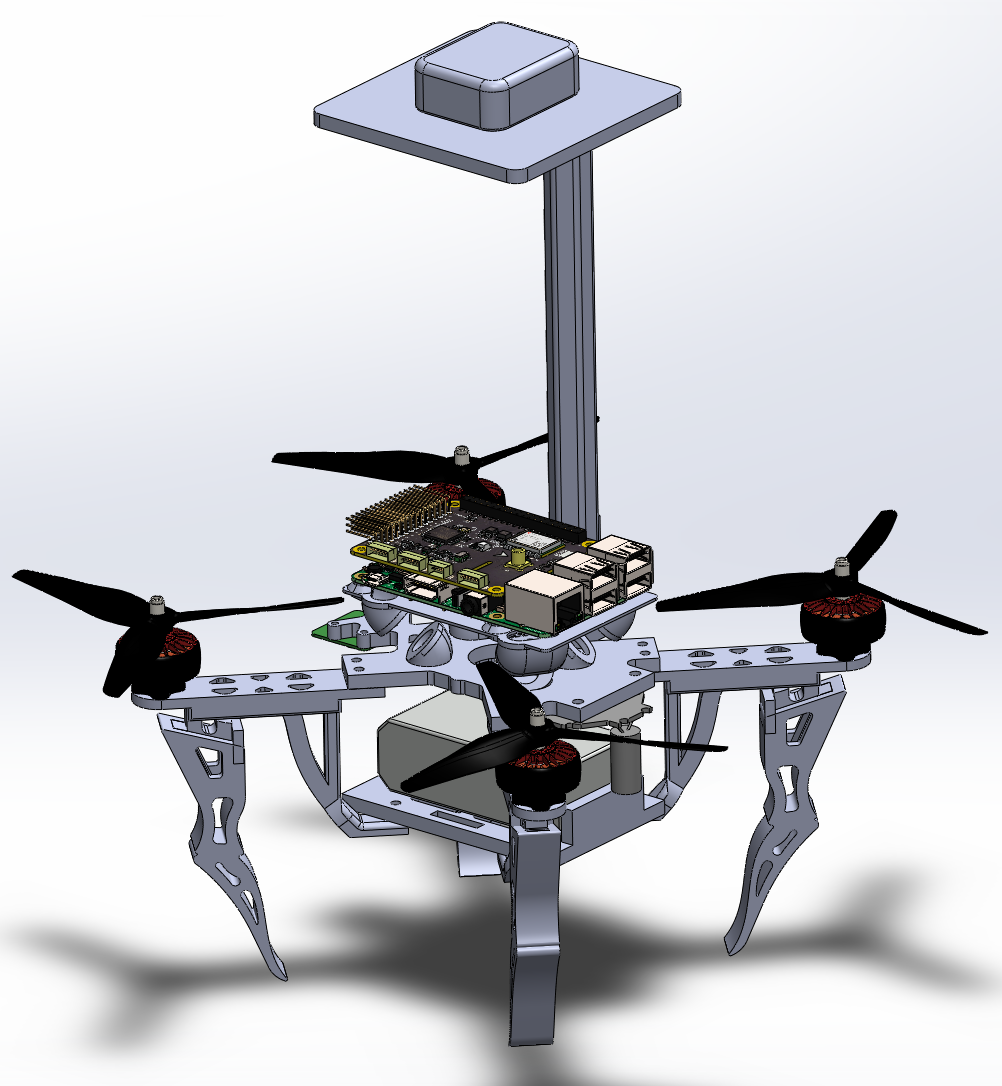
\includegraphics[width=0.75\textwidth]{Reflection/PrototypeI.png}
  \end{center}
\end{figure}

During this first prototype, the frame was kept small and light due to concerns on takeoff weight. As a result, there were small clearances between the propellors and electronics/wires. The flight controller was also attached to the frame only through a friction fit of 4 dampening balls. 
This first design had multiple issues:
\begin{itemize}
    \item Takeoff was very unstable due to the center of gravity being larger on one side of drone due to the weight of the mast being on one side only. This is especially evident in \nameref{fig:PrototypeI}.
    \item Landing legs did not distribute the landing force directly upwards, instead distributing the force at an angle and pushing against a weaker plastic extrusion.
\end{itemize}
After the first flight, catastrophic damage occurred to most components upon a crash:
\begin{itemize}
    \item Mast broke first on flipped landing.
    \item Flight controller separated from the frame, leading to wires not being properly secured.
    \item Many wires then got cut by propellors.
    \item Frame arms were not well reinforced, causing many thinner sections to break.
\end{itemize}
Flight logs were analyzed to verify correct performance. Analysis determined that the error resulted from unstable compass readings due to indoor testing near metallic cabinets. 

\clearpage

\subsubsection{Prototype II}

\begin{figure}[h!]
  \begin{center} 
  \caption{Prototype II}
  \label{fig:PrototypeII}
        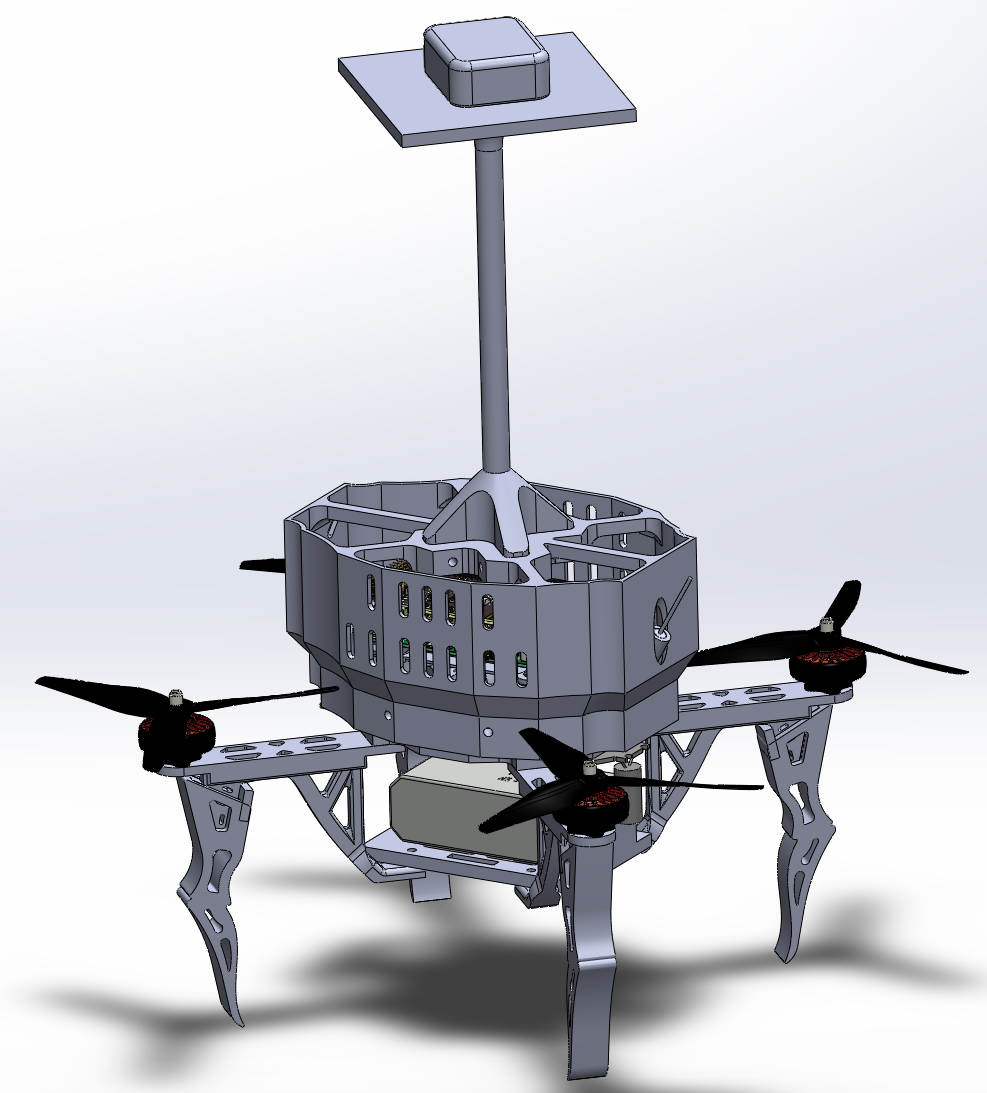
\includegraphics[width=0.75\textwidth]{Reflection/PrototypeII.png}
  \end{center}
\end{figure}

The main lesson from the previous prototype was to provide a proper enclosure for the electronics and to redistribute the mast weight. Takeoff was also achieved with throttle as ~30\%, thus eliminating any weight concerns. Thus, the main change consisted of adding an enclosure and redoing the mast to attach onto the center of the enclosure. To facilitate the additional enclosure, frame size also increased by 10mm. Landing legs were also modified to have ground force directed straight up, greatly improving durability when landing.

Overall, this prototype produced a stable flight for hover. However, the mast still breaks when the drone flips over during landing. Takeoff is also a bit unstable still as it has a tendency to lean on one side, before leveling itself once airborne. Landing is also not ideal as it frequently tips over during landing. Final test of this prototype resulted in another catastrophic damage, where a 23m drop test was unintentionally conducted. This resulted in almost all parts of the frame being broken, and a few wires cut. However, the motors, flight controller, and other electronics were undamaged. Once again, the flight logs were analyzed. Although initially suspected to be an issue in vibrations affecting the IMU, they were found to be within acceptable ranges with no clipping occurring before the crash. The log of vibration values are found in \nameref{fig:vibLevels}. Investigating the battery levels indicated that the battery voltages were inconsistent. Thus, battery voltages and currents were recalibrated. However, this was unlikely to be the source of the crash, and it was determined that the cause was determined to be an unexpected vertical speed of 3m/s followed by an unnecessary emergency stop, resulting in motors cutting off at 23m and entering free fall. No software issues were found, as all commands were given by the Operator through a radio controller. Thus, it was concluded to be an operator error.

\begin{figure}[h!]
  \begin{center} 
  \caption{Vibration Levels}
  \label{fig:vibLevels}
        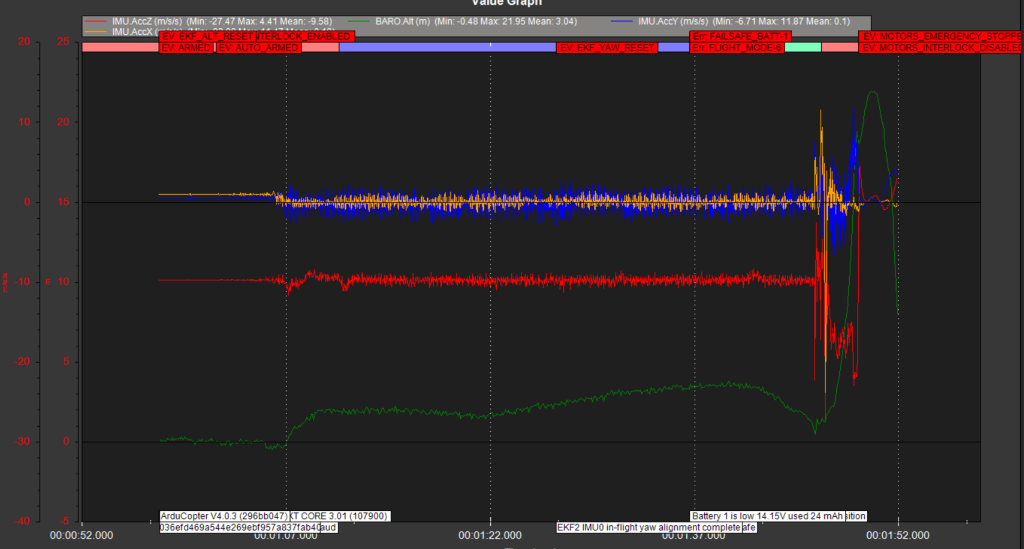
\includegraphics[width=0.75\textwidth]{Reflection/VibrationLogs.png}
  \end{center}
\end{figure}

\clearpage

\subsubsection{Prototype III}

\begin{figure}[h!]
  \begin{center} 
  \caption{Prototype III}
  \label{fig:PrototypeIII}
        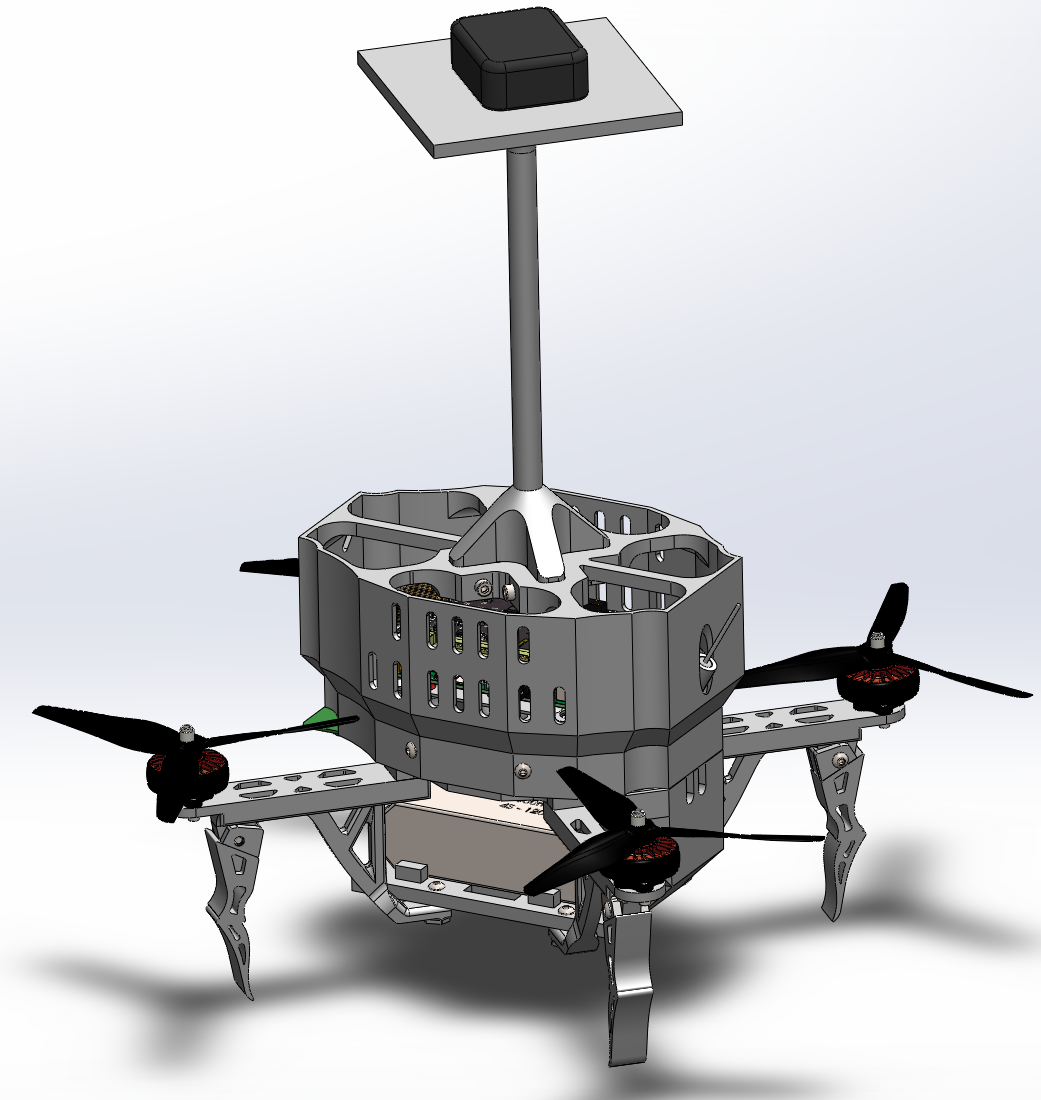
\includegraphics[width=0.75\textwidth]{Reflection/PrototypeIII.png}
  \end{center}
\end{figure}

The main changes in this prototype are correcting the center of mass and improving the sturdiness of the mast. Mass properties of all components were updated within CAD, and battery location was moved to produce central center of gravity. This greatly aided in takeoff by removing previous tendency of leaning during takeoff. The mast was reinforced with a steel rod in the center to prevent shear forces from acting on the plastic mast. This is further shown within \nameref{fig:mastSupport}. The new design significantly improved the durability and can handle multiple crashes and flipping without breaking. On more severe crashes, the steel rod itself bent without the mast disconnecting from the frame. The steel rod was then manually straightened again for repairs.

\begin{figure}[h!]
  \begin{center} 
  \caption{Reinforced Mast}
  \label{fig:mastSupport}
        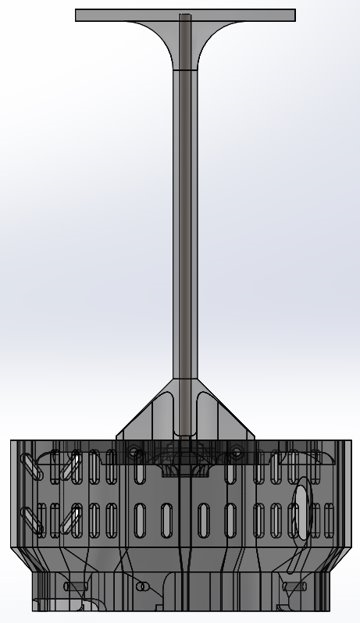
\includegraphics[width=0.35\textwidth]{Reflection/ReinforcedMast.png}
  \end{center}
\end{figure}

\clearpage

An additional thin wall was also created between the base plates to provide increased protection of the ESC from dirt during landing/crashes.
To minimize the tendency to flip over during landing, the center of gravity was modified to be closer to the ground, which was achieved by reducing the length of the landing legs. The joint between the landing legs and frame arm was also redone to use a single nut and bolt as opposed to two zip ties to facilitate repairs and maintenance. This is shown within \nameref{fig:legJoint}.

\begin{figure}[h!]
  \begin{center} 
  \caption{Leg Joint Redesign (Old on Left, New on Right)}
  \label{fig:legJoint}
        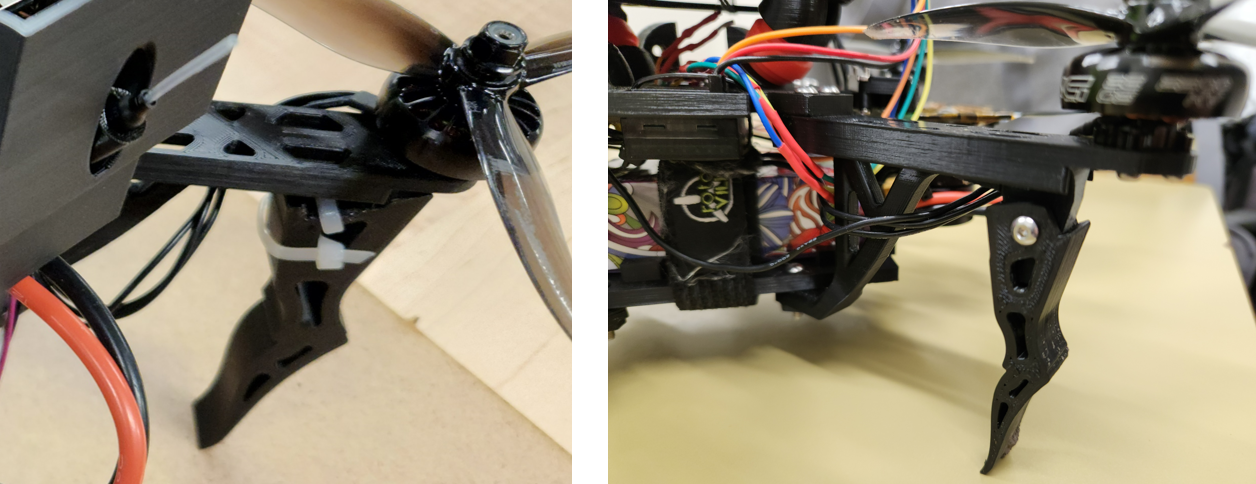
\includegraphics[width=1\textwidth]{Reflection/LegJoint.png}
  \end{center}
\end{figure}

Implementing these changes resulted in significantly more stable takeoff and landing, and drastically improved mast durability. Crashes from ~2m resulted in only the frame arm breaking in the lateral direction. Repairs of the frame arm consisted of reattaching the motors and base plates to the replacement arm. 
However, the on-board camera was found to produce a pink tint during the day due to the lack of an IR filter on the lens. Although this does not occur within indoor environments or during the evening, this would limit the operation of the drone.

\clearpage

\subsubsection{Prototype IV}

\begin{figure}[h!]
  \begin{center} 
  \caption{Prototype IV}
  \label{fig:PrototypeIV}
        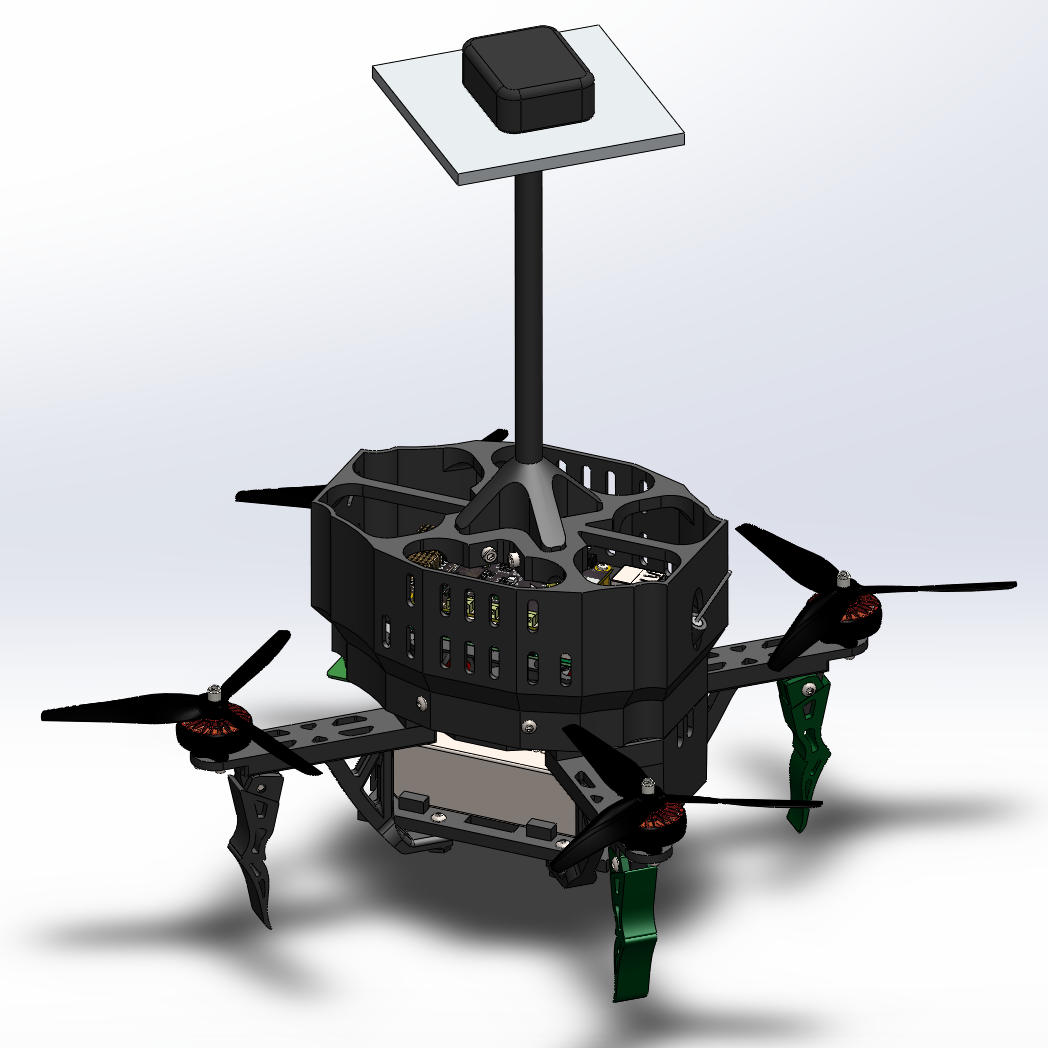
\includegraphics[width=0.75\textwidth]{Reflection/PrototypeIV.png}
  \end{center}
\end{figure}

The focus of the final prototype was to improve the durability of the frame arms, as they are time consuming to replace and print. 3D printed parts have a key limitation of having low shear strength along the layer heights (z direction). Shear strengths along the x and y direction are much larger in comparison.
Based on previous damages to the frame arm, all of the damage has resulted in between the layer heights, thus indicating that this limitation is the cause of previous breakages. Thus, the print orientation was modified by 90 degrees such that the main forces encountered during flight and landing are forces in the x and y direction, which 3D printed parts are stronger in. Although post print processing time is increased due to the additional printing supports required, the durability is greatly increased.
On another crash at 2.5m, the frame arm is undamaged with the landing leg breaking instead at the joint. This is the ideal breakage point as the landing leg can be replaced within a few minutes with only a single bolt and nut.
A new on-board camera was also used that has an IR filter, allowing for clearer images during the day. However, due to the different mounting hole dimensions, a camera mount adaptor was designed to mount the new camera.

\clearpage

\subsection{Visual Perception}
The visual perception development was split into two main parts: the Satellite Maps and its corresponding conversions, and teh segmentation algorithms.

\subsubsection{Satellite Maps and Conversions}
Development initially started with Yandex maps for satellite imagery. Although images could be retrieved at specified longitude and latitude coordinates and then analyzed, there were issues with extracting longitude and latitude coordinates from the pixels within the image. This is due to the elliptical projection method implemented by Yandex. This caused linear interpolation between known coordinates to produce unacceptable accuracy, with values differing by 1-2m.

The next iteration used Google Earth API for satellite imagery. Spherical projection method was implemented by the API, allowing for more accurate linear interpolation between known coordinates. This resulted in under a meter accuracy during conversions between pixels to global coordinates of longitude and latitude. The retrieved images consists of stitching together a 3x3 grid of 640x640 images to produce a 1920x1920 resolution image of high zoom. An example of such can be found in \nameref{fig:StitchedImage}.

\begin{figure}[h!]
  \begin{center} 
  \caption{Stitched Satellite Image}
  \label{fig:StitchedImage}
        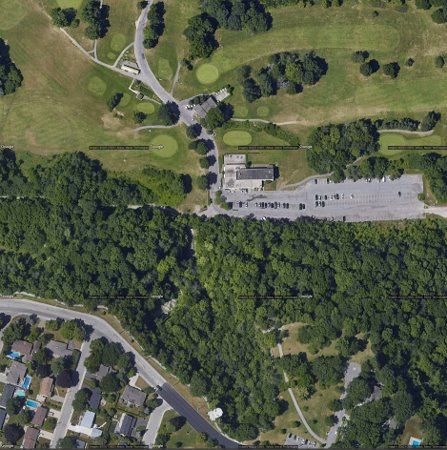
\includegraphics[width=0.75\textwidth]{Reflection/StitchedImage.png}
  \end{center}
\end{figure}

\clearpage

\subsubsection{Segmentation Algorithms}
Development started with applying Canny Edge Detection onto the image to determine contours and grouped contours together into shapes using morphological operations such as dilation and erosion.
However, the result had too much noise and too many edges. Only interested in edges between nature and parking lot boundaries.
Next iteration applied a HSV thresholding filter onto the image to binarize the image. From there, marker-based watershed segmentation was applied to extract the blobs that would then be classified. Classification was conducted by overlaying the blob onto the original image to determine if it is nature, parking lot, or occupied, based on the colour. 
An example of the segmentation is shown in \nameref{fig:SegmentedParking}.
Although performance was acceptable in test cases, testing with a wider variety of images through Google Earth produced less optimal results due to the slight changes in colours. To address this, an additional erosion operation was applied after binarization to reduce noise, and the HSV thresholding ranges were finetuned. This process was facilitated by annotating a wider variety of images and using the Automated KPI Generation tool.

\begin{figure}[h!]
  \begin{center} 
  \caption{Segmented Parking Lot}
  \label{fig:SegmentedParking}
        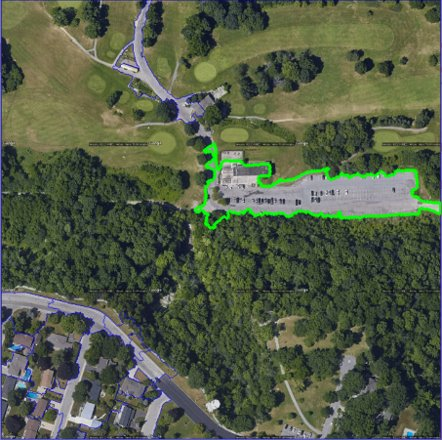
\includegraphics[width=0.75\textwidth]{Reflection/SegmentedParking.png}
  \end{center}
\end{figure}

\clearpage

\subsection{GUI}
\label{subsec:GUI}
Phase II featured an integrated satellite map widget that allowed the user to manipulate the current view by panning and zooming. However, the widget requires internet access in order to retrieve the map. As the drone will be operating in an outdoor environment, internet access would not be provided.
Research on caching the map for future offline use proved to be futile for the widget.
Thus, GUI was updated to display saved images of satellite maps instead of using a widget.
An example map is shown within \nameref{fig:guiMap}.

\begin{figure}[h!]
  \begin{center} 
  \caption{GUI Map}
  \label{fig:guiMap}
        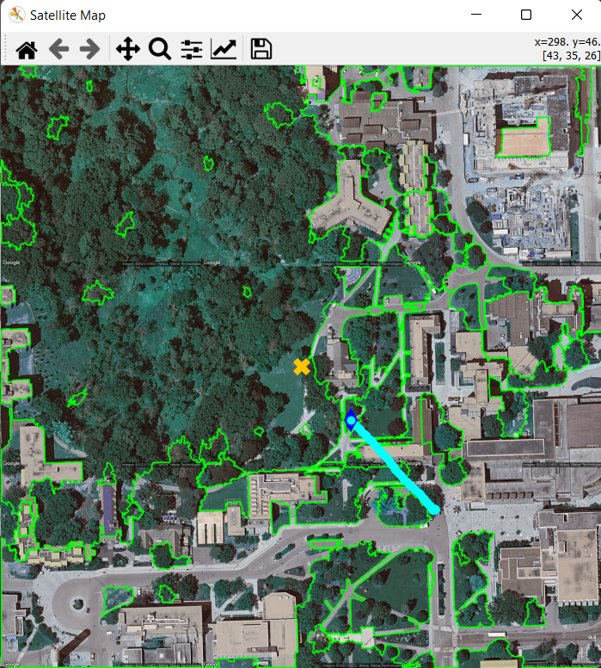
\includegraphics[width=0.75\textwidth]{Reflection/GUIMap.png}
  \end{center}
\end{figure}

\clearpage

To determine which saved image to load, a global coordinate system was established for the GUI, with each point within the coordinate system corresponding to a specific image to load. The point is then selected as the point closest to the drone's current location. Thus, satellite imagery via Google Earth would be retrieved and stitched together for each point within the established global coordinate system prior to operation of the drone. If there is no saved image for the requested point, an error state would be entered.


\section{Design Decisions (LO12)}

The main design considerations are outlined within \nameref{tab:designConsiderations}.

\begin{table}[!h]
\begin{center}
\caption {Design Considerations}
\label{tab:designConsiderations}
\begin{tabular}{ | m{4.7cm} | m{10.7cm} | } 
\hline
Limitation/Constraint & Influence on Decision \\ 
\hline
Time and Expertise Limitation &
    External flight controller hardware used: Navio2. This removes the need to hand pick which sensors to use, and ensures compatibility between the components, and simplifies data communication. There will also be higher quality control on these sensors, as they are packaged as part of a whole product. 
    Similarly, an external autopilot software is used: Ardupilot. This greatly simplifies the control of the drone and provides a high level method of control. There also exists built in methods to communicate with compatible flight controller hardware, such as the Navio2, thus establishing a predetermined interface between the sensors and PWM output for the motors.    \\
\hline
No existing infrastructure required for operation, including internet access. &
    Private LAN network established between Drone and PC for bidirectional communication. Satellite maps must be saved or cached locally without the need for internet. See \nameref{subsec:GUI}.   \\
\hline
Budget limitations. &
    3D printed frame used instead of a carbon fiber frame, which would offer increased durability and reduced weight. The size of the drone was also selected to be small in order to minimize the cost of the motors, batteries, and ESC. However, the disadvantage is that the battery life offers only 5 minutes of flight, whereas larger drones would be able to hold larger batteries, providing up to 30 minutes of flight. There are also no secondary GPS and sensors present. In addition to extra cost, the current frame size has no spare room for additional sensors. No downward facing rangefinders are also present for improved height readings.  \\
\hline
Assumption of operation during non-inclement weather. &
    Product does not need to be operational during high winds or precipitation. Thus, smaller drone is acceptable as it does not need to account for high winds. Electronics also do not need to be fully waterproof and rugged, as it will not operate during precipitation such as snow or rain. Thus, slits in the enclosure exist to promote air circulation for component cooling during operation. However, the  electronics are almost fully covered from the bottom side to better protect against dirt, snow, and puddles when landing.    \\
\hline
Weight constraint of 25kg. &
    Although a constraint, the budget limitation already prevents a drone exceeding 25kg to be created. \\
\hline
\end{tabular}
\end{center}
\end{table}
 

\newpage

\section{Economic Considerations (LO23)}

\indent ParkingLotHawk is a product with the potential to revolutionize the parking lot management industry. The product is specifically designed for organizations with large outdoor parking lots, whose existing monitoring techniques such as walking or cameras are not sufficient during busy periods. Many of these parking lots lack poles for camera attachments, making it difficult to manage parking efficiently. ParkingLotHawk addresses these pain points and can help managers improve efficiency and cost-effectiveness.\\
\indent To successfully market the product, the team must first identify potential customers and understand their unique needs. The team must then showcase how the product can address these needs and provide significant benefits to their business. One potential target audience is property management companies with many parking lots.\\
\indent Currently, the cost of manufacturing a single drone is approximately 750 CAD. In Table \ref{tab:parklothawk-bom}, the cost of direct materials total comes to about 720 CAD. However, this cost could decrease with volume production and the use of different materials. Including an assembly time of 5 hours, printing time of 36 hours, and software and hardware setup time of 2 hours, the total cost comes down to approximately 850 CAD. Considering that the product caters to a niche market and there are few competitors, the team plans to add a 30\% profit margin, pricing ParkingLotHawk at 1105 CAD.\\
\indent In addition, the team plans to charge a 200 CAD annual subscription for each region in which ParkingLotHawk will operate. For example, if a business has multiple parking lots in different locations, then the business would have to pay 200 CAD every year for each parking lot that requires ParkingLotHawk services. This 200 CAD fee allows for further research development of ParkingLotHawk. To ensure profitability, the team must sell about 2-3 ParkingLotHawks to break even. Potential leads within the GTA the team can reach out to for selling ParkingLotHawk are: Go Transit (Pickering GO, Clarkson GO, Streetsville GO and many more), Toronto Transit Commission (TTC) (TTC Finch Lots, TTC Pioneer Village Lot, TTC Kipling Lots and many more) and Oxford Properties Group (Square One Shopping Center, Yorkdale Mall, Scarborough Town Center and many more) amongst many others.


\begin{table}[ht]
\centering
\caption{ParkLotHawk Bill of Materials.}
\label{tab:parklothawk-bom}
\begin{tabular}{lr}
\textbf{Item} & \textbf{Price (CAD)} \\
\hline
Raspberry Pi 3B & 45.20\\
Navio 2 & 383.56\\
Dampening Balls & 6.78\\
Motor & 112.95 \\
Propellers & 4.52 \\
LiPo Battery & 39.54 \\
Electronic Speed Controller (ESC) & 67.8 \\
ArduCamera & 49.10 \\
~36 hours of 3D printing using PLA filament & 11.28 \\
\hline
\textbf{Total} & 721.27 \
\end{tabular}
\end{table}

\section{Reflection on Project Management (LO24)}


\subsection{How Does Your Project Management Compare to Your Development Plan}

\indent Project management and development plan are critical components of any project. The success of a project depends on how well the project management plan is followed, with respect to the team meeting plan, team communication plan, team member roles, and workflow plan. This section will discuss the team's project management compared to the development plan.
\\ \indent Team meeting plan: The team followed the roles assigned to each team member in meetings, and weekly meetings were held as planned. However, some meetings exceeded the planned duration of one hour, which was not ideal. Additionally, some team members were not always prepared for discussion topics due to a lack of preparation time, leading to slower discussions. To mitigate this issue, the members should allocate more time for preparation and consider dividing longer meetings into smaller, more focused sessions. Furthermore, the team must ensure that summaries of the decisions made during meetings are documented to avoid any miscommunication between team members in the future.
\\ \indent Team communication plan: The use of Git Issues as the task tracking software was planned, but due to permission issues, integration with Git and Teams was not possible and led to poor integration with the main communication channel, MS Teams. Instead, the team opted to use Task Planner via Teams to track issues, complete with descriptions, dates, and assignees. OneNote and Teams were used for documents, planning, and communication as initially outlined. Overleaf was added as the document collaboration software for Latex documents, chosen for its online, real-time collaboration feature.
\\ \indent Team member roles: Two administrative roles were identified: Scribe and Leader. Initially, it was planned to have a single person be responsible for each role, with no change over time. However, the team evolved to have different people take on these roles depending on the discussion and other circumstances, leading to more dynamic roles. Domain experts also changed over time as the project progressed and new domain experts were created for each main module to reflect this change.
\\ \indent Workflow plan: The team maintained a production-level master branch with feature branches for development. Automated unit tests were added within the test/ folder to verify the performance of critical requirements, and linters were used as outlined. Git Pull Requests were used for code review before merges, but no continuous integration (CI) was used. Git Issues were not used, in favour of issue tracking within Task Planner. Release tags were used to aid traceability. Although the unit testing framework (GTest, UnitTest, and RosTest) was not used, manual unit tests were created during development. This lack of automatic execution during package building needs to be addressed in future projects. CMake was used for the automatic compilation of new ROS packages and linking, and a custom testing framework to test visual perception modules was created. This testing framework involved using sample images from open-source datasets, in addition to satellite imagery from Google Earth. A wide variety of sample images were selected and annotated manually, using segmentation labels of ParkingLot, Nature, and Occupied. The testing framework is then used to automatically feed in the annotated images and produces an output csv containing ground truth data and the algorithm prediction. The outputs are then analyzed for further iterations of the algorithms.

In conclusion, the team followed some aspects of the development plan while deviating from others due to unforeseen circumstances. The team should allocate more time for preparation, divide longer meetings into smaller, more focused sessions, and ensure that summaries of decisions made during meetings are documented. Additionally, integration of task-tracking software with our main communication channel should be improved, and unit testing framework for automatic execution during package building should be considered. Despite these challenges, the team successfully managed the project and delivered the objectives.


\subsection{What Went Well?}

\\ \indent The project management processes and technologies implemented for this project had several positive outcomes that greatly aided in the successful completion of the project. One of the most useful tools utilized was OneNote, which provided a centralized location for all project notes and planning documents. This allowed for easy access by all team members and ensured that everyone was working from the same information. Overleaf was also highly effective, providing real-time collaboration tools for the team. This allowed for smooth and efficient collaboration on Latex documents, without the risk of conflicts arising from simultaneous edits.
\\ \indent Another positive aspect of the project management was the dynamic team roles that evolved over time. This allowed team members to become experts in the roles that were required at different stages of development, leading to a more agile and responsive team. Additionally, the use of the feature-branch methodology on GitHub was highly effective. This methodology ensured that only production-level code was available on the master branch, while separate feature branches were used for parallel development. This aided in the traceability of features and allowed for faster and more efficient development.
The use of release tags was also useful in measuring major milestones and maintaining an overall history of the project. This ensured that team members were aware of project progress and could identify areas for improvement.
\\ \indent Finally, the custom testing framework developed for the visual perception modules was highly effective in aiding development and tuning of algorithms. The framework allowed for automated key performance generation, which greatly sped up the testing process and provided quantifiable performance values for comparison with different algorithms and tunings. This helped the team to identify and rectify issues quickly and efficiently.
\\ \indent Overall, the project management processes and technologies implemented for this project had many positive outcomes. The use of centralized document sharing and collaboration tools, dynamic team roles, feature-branch methodology, release tags, and custom testing framework all contributed to the successful completion of the project.

\subsection{What Went Wrong?}

As previously mentioned, documentation of meeting decisions not fully documented for reference, leading to miscommunication later on. Although the role of a scribe was maintained, some meeting details were still missed. Meetings sometimes exceeded the allocated time as well, producing long meetings that could be broken up into smaller, more productive meetings. 

Git issues were also not used, causing poor traceability between commits and tasks. The tasks were outlined within the MS Teams Task Planner, but the main method of communication, Teams, was not able to integrate with Github due to permission errors. Thus, this split between Teams and Github caused a non-unified project platform.

The main issues are with respect to testing. Mainly occurring due to the lack of time, testing occurred later in the product lifecycle than ideal, leaving less time to properly integrate the test cases into the workflow.
Unit tests should be created before the development of the modules, and after the creation of the requirements. This allows for testing during the development of the modules, as opposed to testing once the module is completed. The unit tests should also be integrated into the CI pipeline or other automated test methods. 
On the topic of CI, it was not implemented due to insufficient time and the absence of unit tests early on during development. This led to more manual work during merges, requiring manual execution of the created test cases to ensure correctness. 
Unit testing framework was also not used, producing poorer unification of test cases and automated execution. Thus, it was more difficult and time intensive to run and manage all tests when verifying the performance.

\subsection{What Would you Do Differently Next Time?}

\\ \indent For the next project, the team plans to make several changes to their project management approach. Firstly, they will ensure more detailed meeting notes are created by reviewing the notes after each meeting to ensure all important information is included. This will prevent miscommunications later. Secondly, they will produce better integration of issues, tasks, and Git by using Git Issues for discussions regarding design and tasks instead of Task Planner and Microsoft Teams. Meeting minutes will be created on Git issues and related discussion surrounding tasks will be linked to the commits. The commit that closes the issue will then be linked to the issue. This ensures that all task-related work is on a single platform: GitHub and GitHub Projects.
\\ \indent The team will also allocate more time for testing earlier in the product lifecycle. To address the source of mistakes in testing, the team will write a collection of barebones unit tests with the intent to check all requirements after the requirements are developed. At this stage, the unit tests will not be functional. These unit tests will be written using the associated Unit Testing framework, such as GTest for C++, UnitTest for Python, and RosTest for ROS-specific modules. Once modules are decided upon, the collection of unit tests will be modified accordingly with the new modules. The development of these unit tests will begin before the development of the modules to test them as development progresses.
\\ \indent Unit tests will be added to CI and set to run every time a push is made. This will aid in the traceability of bugs and assurance that the module's behaviour meets expectations. At this stage, system tests should also be considered, and any additional test cases should be created and added to the CI. These changes will produce automatic execution of test cases through CI and allow the tests to be used during the development of the modules to aid in development.



\end{document}
